\chapter{Background}\label{sec:Background}
In this section we will go over

\section{Distributed Systems}\label{sec:Distributed Systems}

Significant consequences of distributed systems, Concurrency, Absence of global clock, Failure independency

Heterogeneity • Openness
• Scalability
• Transparency •Failure handling • Concurrency
• Security

importance of models

coordination problem

Synchronous vs. asynchronous systems Asynchronous system
– No assumptions about process execution speeds and/or message delivery delays
– Weak assumption: any system is asynchronous
 Synchronous system
– Relative process speeds and ...
– ...Message delays are bounded

A communication example
– Reliable channels
If P sends a message m to Q and Q does not crash, then Q receives m.
– Quasi-reliable channels
If P sends a message m to Q and both P and Q do not crash, then Q receives m.

– Failstop: a process fails by halting. Once it halts, the process remains in that state. Other processes can detect the failed process.
– Crash: a process fails by halting. Once it halts, the process remains in that state. A failure may or not be detected by other processes.
– Byzantine failures: a process fails by exhibiting arbitrary behavior.
Crash+Link: a link fails by losing some messages, but does not delay, duplicate, or corrupt messages.
– Receive-omission: a process fails by receiving only a subset of the messages sent to it, or by halting (i.e., crashing).
\section{Consensus}\label{sec:Consensus}

The problem of consensus is a fundamental problem in distributed systems: it was first introduced in the early 80s \cite[]{Pease}, \cite[]{Lamport} and since then it remained important in most distributed environment, ranging from more classical server applications to the more recent Blockchains.

Consensus is basically an agreement problem: the goal is to have a set of entities reach an agreement on a value that was previously proposed by (at least) one of those entitities. This definition is quite general, and for a good reason: depending on the different assumptions we make on the system model, there are stronger and weaker types of consensus that can be achieved. 

The three core properties of a consensus protocol are the following:

\begin{itemize}
    \item \textbf{Termination} Eventually every correct process decides on one value
    \item \textbf{Uniform integrity} If a process decides on a value, then this value was proposed by some process
    \item \textbf{Uniform agreement} No two processes decide on a different value
    \end{itemize}

\begin{figure}[htb]
  \centering
  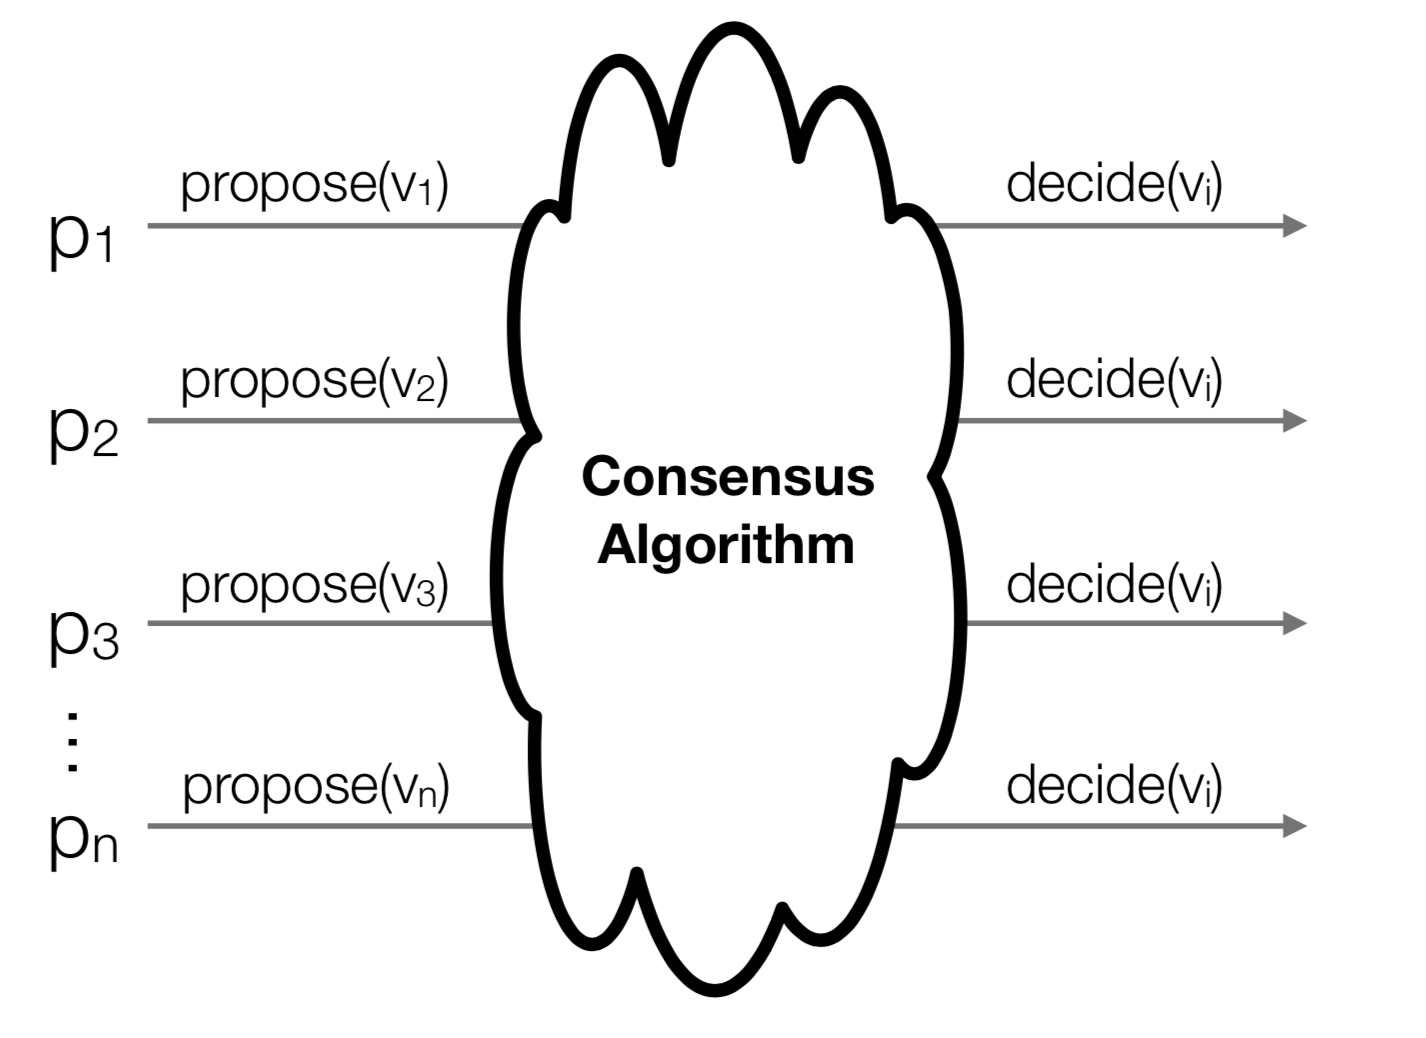
\includegraphics{img/consensus.png}
  \caption[The architecture of the system]{ The architecture of the system. The
    \textit{Viper IDE} and \textit{Viper Debugger} boxes denote, respectively,
    the main Viper extension and the new debugger extension. They both interact,
    independently, with Visual Studio Code. Viper Server is responsible for
    running the verification backends.}
  \label{fig:consensus}
\end{figure}

In this section we will go over some of the more relevant types of consensus, and respective implementations that are able to achieve consensus in the given system models.


\subsection{Synchronous model}\label{sec:Synchronous model}
In a synchronous system model, consensus is quite straightforward to achieve. Let us assume to have a set of $n$ processes, that will be the entities that want to reach a common agreement upon a proposed value. Let us also introduce the primitives used by the processes: each process is able to send and receive messages, through the primitives $send(m)$ and $receive(m)$ respectively, to communicate their intentions to the others. The failure model in a crash failure model, hence a correct process will never crash, while a faulty one eventually will; the number of faulty processes $f$.

Since we are in a synchronous model, we have a bound on the maximum time delay of a message, which means that a process is sure that if a message is sent, it will be received by the receiver before the maximum time delay. This is a quite strong and unrealistic model, but it makes the algorithm to solve consensus quite simple.

Let us have the algorithm proceed in rounds, where each round is as follows:
\begin{enumerate}
    \item Each process sends to all other processes a message containing information about its state.
    \item At the end of the round, after the maximum time bound, processes will have received a set of messages from a subset of all processes.
    \item The processes will then use the received messages together with its current state to reach a new state.
\end{enumerate}

The state can be simply a set values received until that moment, with the initial set containing only our own proposed value. Also, in a round a process can receive only a subset of messages from the other processes, since we can have up to $f$ faulty processes.

After $f+1$ rounds, we can be certain that each correct process will have enough information to deterministically decide on a single proposed value, and therefore reach consensus. This is because if we have a round where no process fails, then every process will receive all other values, and therefore we will be able to decide on a value. Also, since we have at most $f$ faulty processes, we can have at most $f$ rounds with a failing process. Therefore, we can be certain that $f+1$ rounds will be enough to reach agreement.

[should I put the lemmas properly?]

\subsection{Asynchronous model}\label{sec:Asynchronous model}
In this model, we have no bounds on process speed and maximum message delays; this means that a process if or when a message will be received by the other processes. This is a much weaker model compared to the previous one, and as a matter of fact it is proven that consensus cannot be solved in such a model [FLP proof].

\subsection{Alternative models}\label{sec:Alternative models}
The synchronous model allows us to solve consensus, but it's too strong of a model to be of any practical use. The asynchronous model cannot solve consensus. Therefore, we either have to find a system model that is weaker than synchronous and stronger than asynchronous, or we have to weaken the problem.

An alternative system model would be a partially-synchronous one, where the messages are asynchronous up to a GST (Global Stabilization Time), after which we can assume communication to become synchronous.

Another option is to still use an asynchronous system, but to also elect a process to be the leader and guide the whole decision procedure; an example of such an algorithm is Paxos, which is presented in the next section.

We could have failure detectors (which can be used with varying levels of completeness and accuracy), which could allow us to figure out when a process has failed, and therefore stoping us from waiting indefinitely for a message like in the basic asynchronous model.

An example of weaker problem definition would be to allow, for example, to have multiple values decided.

\section{Paxos}\label{sec:Paxos}
Paxos is an algorithm to achieve consensus that relies on an asynchronous system model, which makes it particularly interesting for real world application where we don't have completely reliable communication channels. To achieve this, the Paxos algorithm needs to elect one process as a leader that will act as a coordinator during the various phases of the protocol.

In Paxos, there are four types of process roles:
\begin{itemize}
  \item \textbf{Proposers} the processes that want to propose a value to be decided
  \item \textbf{Acceptors} the processes that take part in the voting part of the protocol; a quorum of acceptors is needed
  \item \textbf{Learners} the processes that, at the end of the algorithm, will be notified about the value decided by the algorithm
  \item \textbf{Leader} the process that acts as a coordinator
\end{itemize}

The election of the leader can be achieved in many different ways, as long as there is a point after which we have a unique correct process that is identified by the other processes as the leader.

The algorithm is divided into tree phases. During phase 1, a proposer that wants to propose a new value sends a new arbitrary value c-rnd higher than any previous c-rnd to the acceptors, so that all of them know that this is the most recent proposal attempt. Each acceptor, if the received c-rnd is truly the highest one it has received, replies to the proposer with its current state (rnd, v-rnd, v-val) so that the proposer know if there was already a previous proposed value, or if the proposer is allowed to propose its own.

In phase 2, once the proposer has received a reply from a quorum of acceptors, it checks if there was any acceptor that had previously voted for a value, and if this is the case, it picks the most recent one as the value to propose. If instead no acceptor had previously voted for a value, the proposer will be able to propose its own value. The proposer will then send to the acceptors the actual value to be proposed.
The acceptors, if the message of the proposer is still the most recent on-going proposal, will send back a message as an acknowledgement back to the proposer.

In phase 3, once the proposer receives again a quorum of replies from the acceptors, will be allowed to send to the learners the newly decided value.

The pseudo-code for the phases is as follows:
\begin{verbatim}
  c-rnd : highest-numbered round the process has started
c-val : value the process has picked for round c-rnd
% rnd : highest-numbered round the acceptor has participated, initially 0 v -rnd : highest-numbered round the acceptor has cast a vote, initially 0 v-val : value voted by the acceptor in round v-rnd, initially null
% To propose value v:
% increase c-rnd to an arbitrary unique value send (PHASE 1A, c-rnd) to acceptors
% upon receiving (PHASE 1A, c-rnd) from proposer if c-rnd > rnd then
% rnd ← c-rnd
% send (PHASE 1B, rnd, v-rnd, v-val) to proposer
% Phase 1B Phase 1A Acceptor Proposer
% upon receiving (PHASE 1B, rnd, v-rnd, v-val) from Qa such that c-rnd = rnd k ← largest v-rnd value received
% V ← set of (v-rnd,v-val) received with v-rnd = k
% if k = 0 then let c-val be v
% else c-val ← the only v-val in V
% send (PHASE 2A, c-rnd, c-val) to acceptors
% upon receiving (PHASE 2A, c-rnd, c-val) from proposer if c-rnd >= rnd then
% v-rnd ← c-rnd
% v-val ← c-val
% send (PHASE 2B, v-rnd, v-val) to proposer
% upon receiving (PHASE 2B, v-rnd, v-val) from Qa
% if for all received messages: v-rnd = c-rnd then
% send (DECISION, v-val) to learners
upon receiving (PHASE 1B, rnd, v-rnd, v-val) from Qa such that c-rnd = rnd k ← largest v-rnd value received
V ← set of (v-rnd,v-val) received with v-rnd = k
if k = 0 then let c-val be v
else c-val ← the only v-val in V
send (PHASE 2A, c-rnd, c-val) to acceptors
upon receiving (PHASE 2A, c-rnd, c-val) from proposer if c-rnd >= rnd then
v-rnd ← c-rnd
v-val ← c-val
send (PHASE 2B, v-rnd, v-val) to proposer
upon receiving (PHASE 2B, v-rnd, v-val) from Qa
if for all received messages: v-rnd = c-rnd then
send (DECISION, v-val) to learners
\end{verbatim}

\begin{itemize}
  \item \textbf{Termination} Eventually every correct process decides on one value
  \item \textbf{Uniform integrity} If a process decides on a value, then this value was proposed by some process
  \item \textbf{Uniform agreement} No two processes decide on a different value
  \end{itemize}

\begin{figure}[htb]
\centering
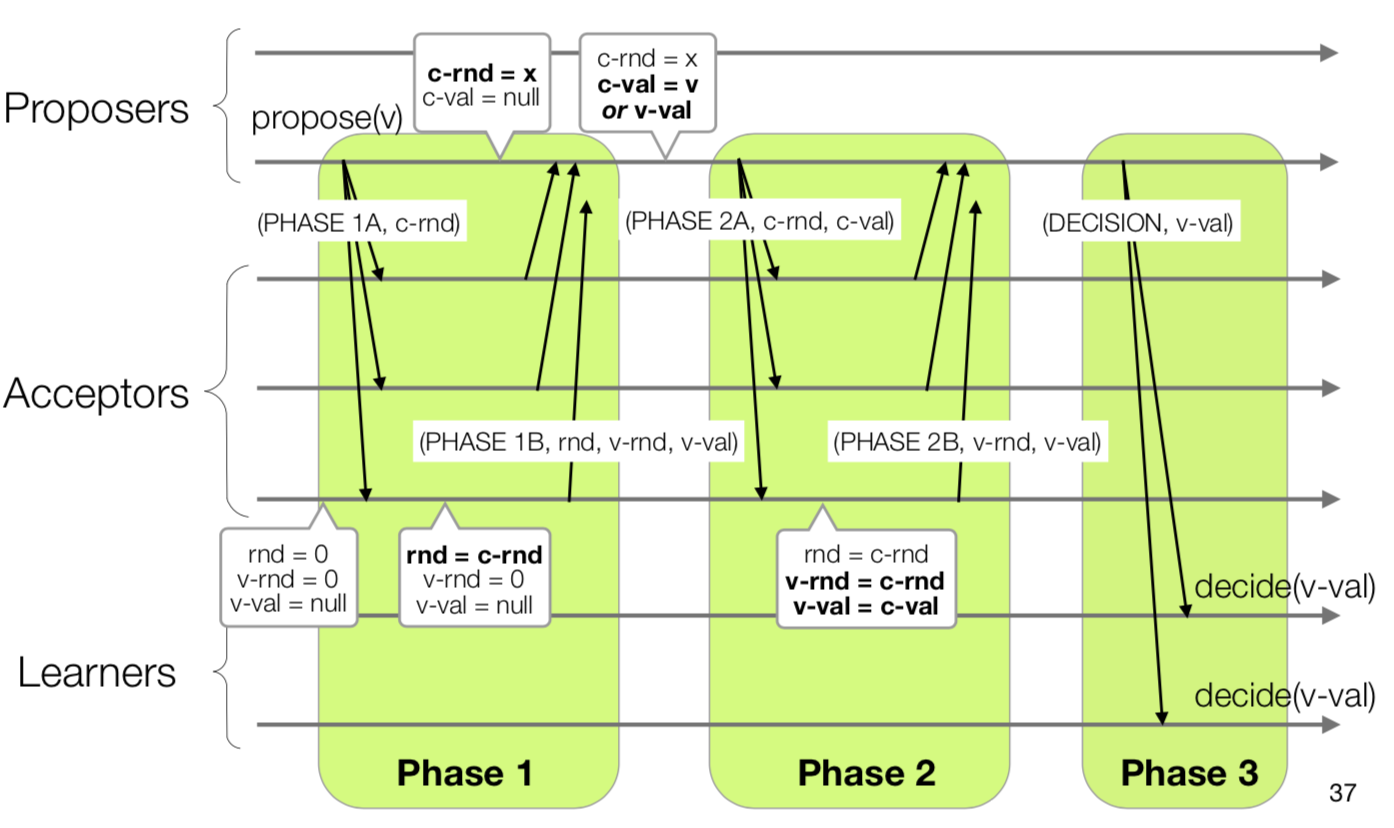
\includegraphics{img/paxos.png}
\caption[The architecture of the system]{ The architecture of the system. The
  \textit{Viper IDE} and \textit{Viper Debugger} boxes denote, respectively,
  the main Viper extension and the new debugger extension. They both interact,
  independently, with Visual Studio Code. Viper Server is responsible for
  running the verification backends.}
\label{fig:paxos}
\end{figure}